g%=======================================================================================%
\chapter{Concluding Remarks: Where next for Molecular Studies of CFTR.}
\label{chap:conclusion}
\chapquote {We have more problems than hands. }{- Eduardo Perozo (personal communication)}

As figure \ref{CF_life_expectancy} demonstrates, basic science discoveries concerning CF have had a direct effect on the life expectancy of patients. The work in this thesis is a small example of how abstract physical models, such as those outlined in \ref{chap:methods}, can be applied to help real patients in a community such as allowing patients in Sydney Children's hospital to access medications which could add decades to their life span. We are entering an exciting era of biophysical research where advances in theoretical methods, computing power and experimental techniques are beginning to drive advances in each other at a frenetic pace. An example can be seen in the development of Alphafold. The maturation of cryoEM allowed the discovery of new protein folds which Alphafold's machine learning algorithms could then learn from. Now that the algorithm had these folds in hand it could predict entire proteomes. This now means that structural biologists can use the predictions of alphafold to solve even more structures more quickly. Eventually, more and more of the experimental work currently involved in biology will move onto the silicon chip, while experimental techniques will advance in other areas. Similarly, the theoretical model argued for in this thesis will eventually allow for patient assessments to be made \textit{in silico}

The preceeding chapters have given technical and molecular details about how Cystic Fibrosis is caused by rare mutations and further demonstrated that these mutations may be treated by existing small molecule drugs. The unique molecular fingerprint of each mutation indicates that in order to deliver better outcomes to patients a more personalised approach is necessary to the choice of medication. 

In order to tie these results together, in this chapter I will propose a conceptual framework which explains how these drugs are able to treat such diverse molecular phenotypes. This model would appear to suggest that patients with rare missense mutations would be more likely to respond to respond to CFTR modulators. The implications of this model are also likely to inform the design of future generations of CFTR modulators. 

The model we will propose raises the importance of some outstanding fundamental questions about CFTRs structure and function. Some of these questions simulations are uniquely placed to answer and we will outline some studies to address them. 

As such, the areas which deserve the most attention for molecular studies of CFTR are to address the controversies surrounding its structure and elucidate the action of drug binding. Together these will allow a clearer understanding of CFTRs function in health and misfunction in disease, enableing more targeted drug development. Current generation modulators have been identified using high throughput screening, the new generation of high computational power, artificial intelligence and structural data will allow a more targeted, perhaps even mutation specific approach to the design of new modulators.

\section{Addressing Controversies Surrounding the Structure of CFTR}
The most recent structure of human CFTR in a phosphorylated environment has some interesting features which have lead to some controversies in the literature. After spending significant time researching them I have conducted an extensive literature review in order to learn more about of these concerns. The released structure of activated, human CFTR has two features that have caused some in the CF field to suggest issues with this structure. Firstly, this structure is not sufficiently open to conduct chloride ions. Chloride ions have a diameter of 1.7$\AA$ while the structure has a constriction of 1.1$\AA$\cite{Zhang2018}. So, there must be some level of conformational changes, even if chloride were to move through the channel completely dehydrated. This becomes even more of an issue when considers the experimental evidence where much larger anionic species such as bicarbonate and glutathione were shown to permeate through the channel\cite{kogan2003}. This suggests that there is a much larger conformation which has not been observed experimentally or in simulations. This was the motivation for chapter \ref{chap:opening} of this thesis. Some studies have been performed in order to study the possible permeation paths of chloride but they were usually not carried out on hCFTR or have not addressed the pressing question of how larger ions might permeate the channel \cite{farkas2020, zeng2021}. Bicarbonate in particular is of great physiological importance as there is a high correlation between the channel's ability to permeate bicarbonate and the pancreatic sufficiency of a patient carrying the mutation \cite{}. In light of this, structural knowledge of a fully open conformation of CFTR is critical to a personalised approach to the treatment of CFTR.

The second and harder to resolve controversy concern the role of TM8. This transmembrane helix has an unusual bend in the middle of the plasma membrane. This is not something seen before in ABC transporters of this type. So it has led to some open questions as to how this bend might contribute to the function of the channel \textit{or} how it might be an artifact of the imaging process. For the former case, the structural biologists in the Chen lab proposed a mechanism whereby the upper hinge of TM8 swings 55$^o$ during the transition to the open state. This mechanism would give justification of the pathogenesis of certain mutaions such as L927P. 

The arguments for the bend in the helix appear to be unphysical. In cryoEM structures, we can observe that the bent conformation is stabilised by salt bridges R347-D924 and E873-R933. The former bond has been well studied experimentally and was expected in the 3d structure. Additionally, all hydrogen bonds along the in the bent helix are . Been observed to be stable in MD \cite{corradi2018} .  is energetically stable.

However, there are still some unanswered questions for the discrepancy between the solved human and solved chicken structures. Certain salt bridges are not present in the latter structure and so single channel electrophysiology experiments may be able to resolve these issues. For example, in 6MSM, the human structure of CFTR there is a salt bridge between amino acids 933 and D873 which is not present in the chCFTR structures. This bond is also present in the zCFTR structure 5W81. If a charge swapped mutant such as R933E/E873R restores WT-like gating behaviour to the channel it would be  strong evidence for the unwound conformation of TM8. 

The two proposed conformations also have vastly different ion permeation pathways, and so blockers engineered to target one conformatoin over the other would also go a long way to answering these questions. The available evidence strongly favors the R334 pathway between TM1 and TM6. Such as experiments to  demonstrate the blockage of current with zinc have shown that mutations to R334 strongly suggest that chloride permeates along this route. Additionally, trhere are several disease causing mutations in the region surrounding R334, such as R334W, R117H, E116K, D110H, I336K\cite{cftr2}. This permeation route also explains the rationale behind the gain of function mutation F337A \cite{}. Determining which model is correct has wide implications for creating the next generation of mutation targeted potentiator class drugs.

\cite{gao2015} also concluded that the chloride opening lined TM6. The findings that TM1 and TM6 move apart form eachother in \cite{negoda2018} also support this conclusion (this is consistent with our open model). Which is more consistent with the 6MSM model than the chicken structure.

The chicken structure has undermised NBDs, this is inconsistent with biochemical assays that dimerisation is tightly coupled to the dimerisation of NBDs\cite{vergani2005, yeh2021}.

Mutagenesis studies of the outer pore would strongly support the Chen structure over the chicken streucture. In particular, Paul Linsdell performed very careful experiments to measure blockage chloride blockage and found that several residues play an important role in the permeation of chloride in the outer pore. In the chicken structure these residues are occluded and far from the chloride permeation pathway. However, in the Chen structure they appear to play an important role in the permeation of chloride. This will be discussed in detail in \ref{chap:opening}.

A study assessing the accuracy of Alphafold's predictions of transmembrane protein structures found an intersting result. When alphafold made predictions that involved the use of templates it predicts the unwound conformation of TM8. On the other hand, when templates are removed from alphafolds predictions it predicts a straight TM8 conformation, very similar to that found in chCFTR. The authors of this study suggested the reason for the discrepancy was due to the use of detergents in the deteremination of the structure of hCFTR. However, careful reading of cryo-EM literature reveals no examples where the use of detergents has resulted in such drastic conformational changes. One of the few examples where both detergents and native-like nanodisks were used to determine the structure of a protein are the determinations of the structure of TRPV1. These studies revealed no difference to the backbone helices but did suggest important information about the importance of different interactions with lipids\cite{gao2016}. A lot of work has been performed in order to create detergents which reflect a native lipid environment and these are the species that were used in the determination of the human CFTR structure (albeit at a higher than optimal concentration) \cite{gao2016, Zhang2018, kampjut2021}. 

The authors of the chCFTR paper suggested that the different expression systems used in the two studies could be the reason for the discrepancy between the two systems, due it their different post translational processing apparatus. Although both groups used mammalian cell lines the chCFTR paper used hamster? cells \cite{aleksandrov2015} and the Chen lab used HEK293S cells. The chicken structure also underwent significant mutations in order to be locked open and imaged. The regulatory insertion was deleted in order to aid in the purification of the protein. 

Figure \ref{} shows the large diversity of structures in type IV ABC transporters, many of which also exhibit bends within transmembrane helices\cite{thomas2020}. Although none of these structures exhibit such a bend in TM8 specifically, the 

\ref{negoda2019} gives strong evidence that TM8 must line the conduction pore. Due to its proximity to F337 and other pore lining amino acids. This is more consistent with the Chen structure than the chicken structure where 337 is far from the conduction pore.

\section{A Physics Motivated Model for the Molecular Modulation of Mutant CFTR }
In chapter \ref{chap:I37R}, \ref{chap:R352Q}, \ref{chap:S945L} and \ref{chap:opening} we have analysed a disease causing mutation in detail in order to understand \textit{how} they cause CFTR to misfunction. What we have found is a large diversity of molecular phenotypes which may cause disease. What is thus remarkable is that the \textit{in vitro} component of these papers all demonstrate that these mutations are responding to the same drugs, albeit with differing efficacies.



The above model in figure \ref{drug_action_model} gives a rational, physical basis for the wide range of molecular phenotypes that CFTR modulators appear capable of treating. This same model would appear to argue that for most missense mutations we would expect them to respond to some sort of CFTR modulator.

\section{A Physics Motivated Approach to Precision Medicine in Cystic Fibrosis}


In recent years there have been a slew of rare CF-causing genotypes discovered in populations with low rates of Cystic Fibrosis compared to Caucasians. These genotypes from Asia and the Middle East are often ultra-rare leading to poor outcomes for these patients, particular lb when local health care is sub standard \cite{}. 



\begin{figure}
	\begin{center}
	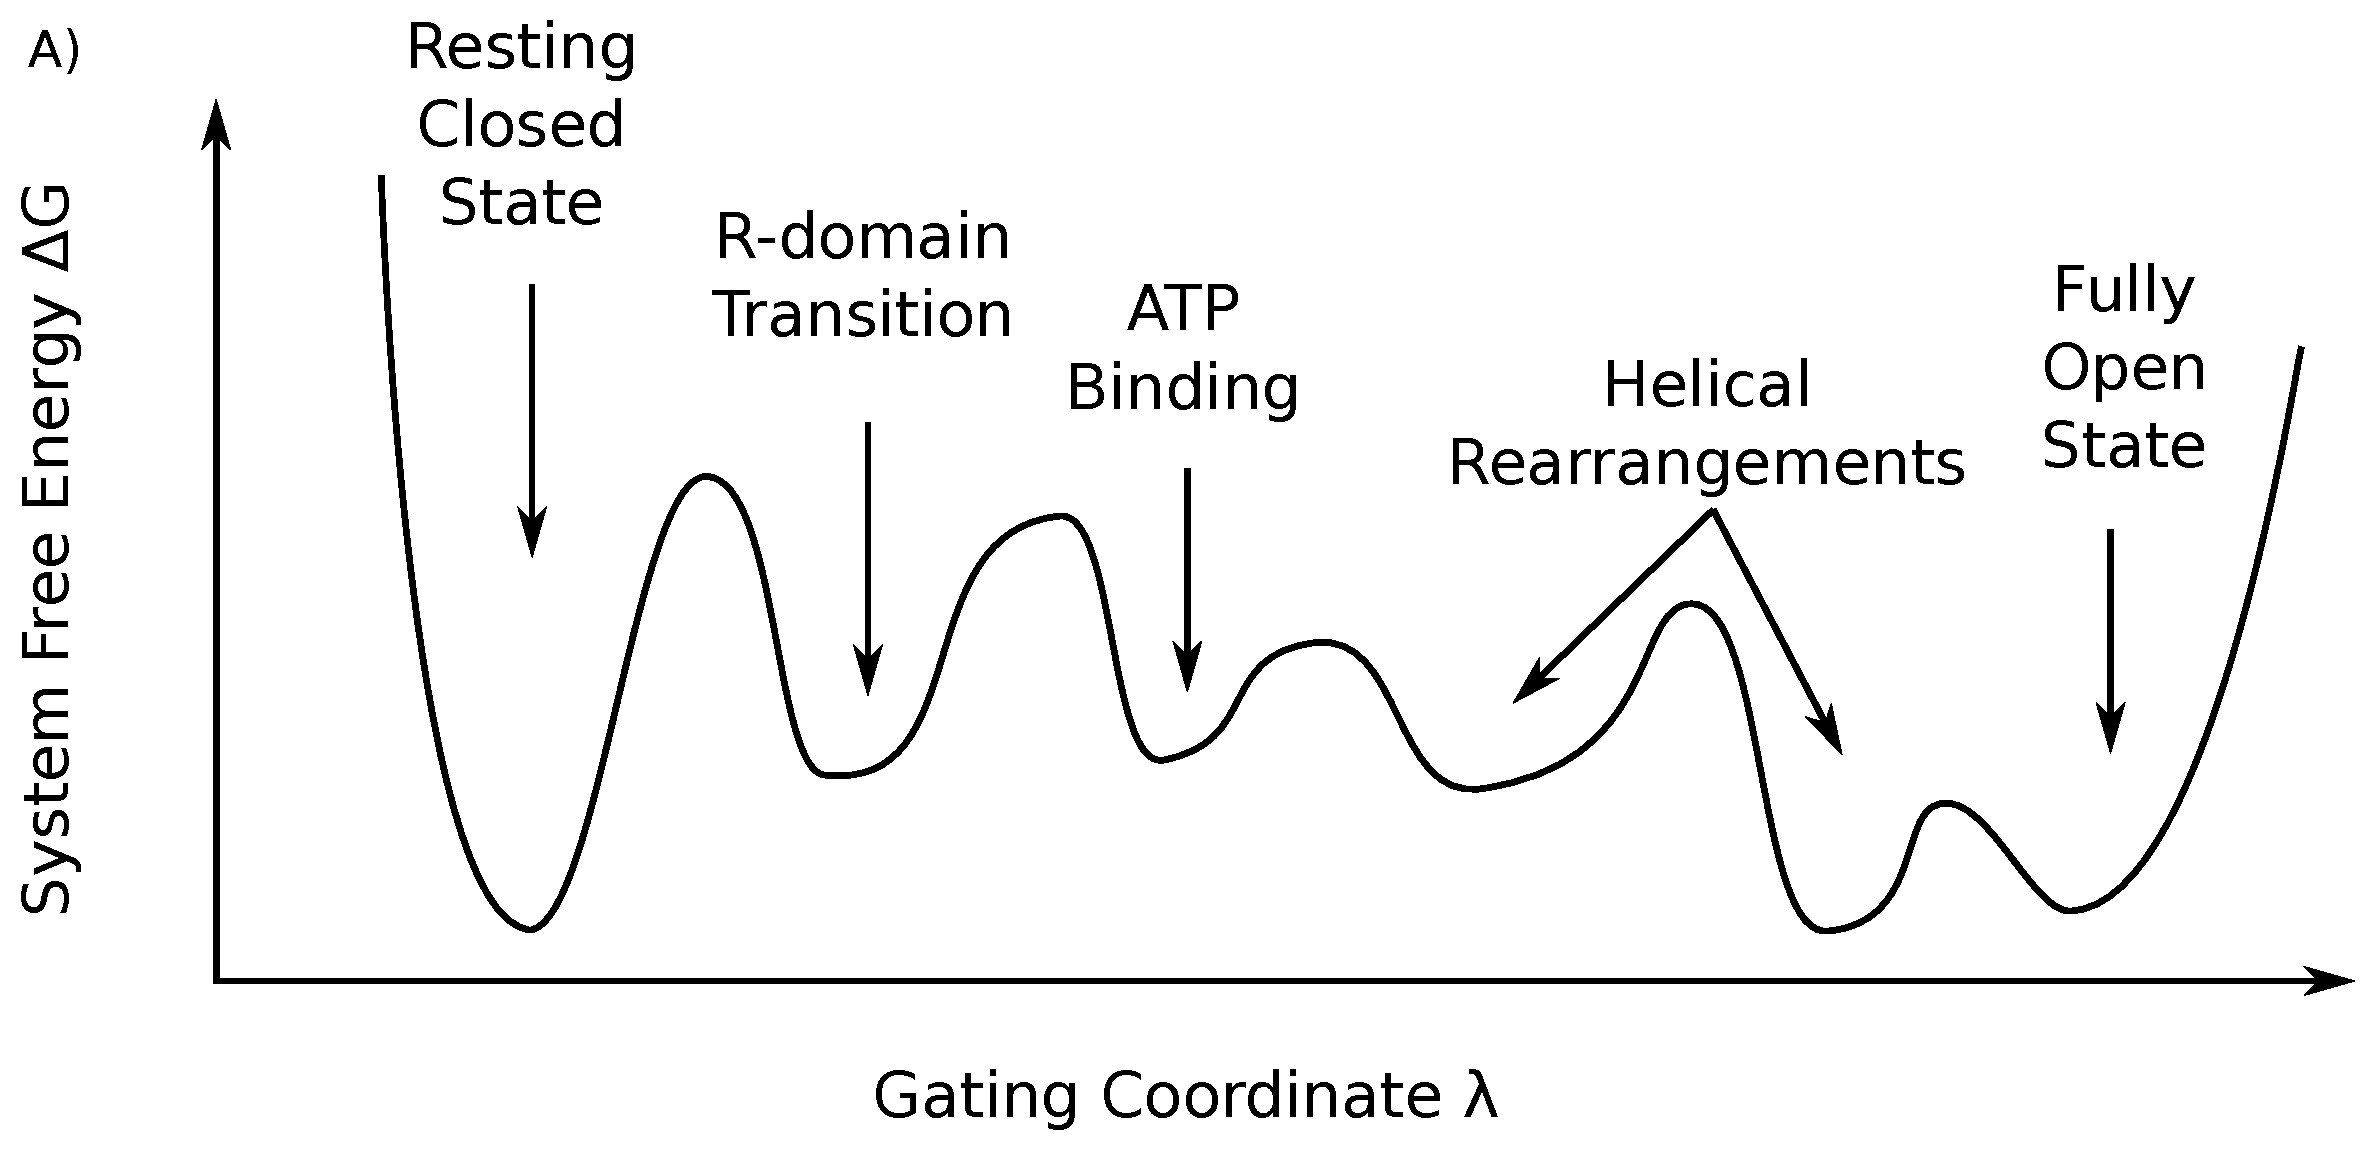
\includegraphics[width=\textwidth]{figures/drug_landscape_1.pdf}\\
	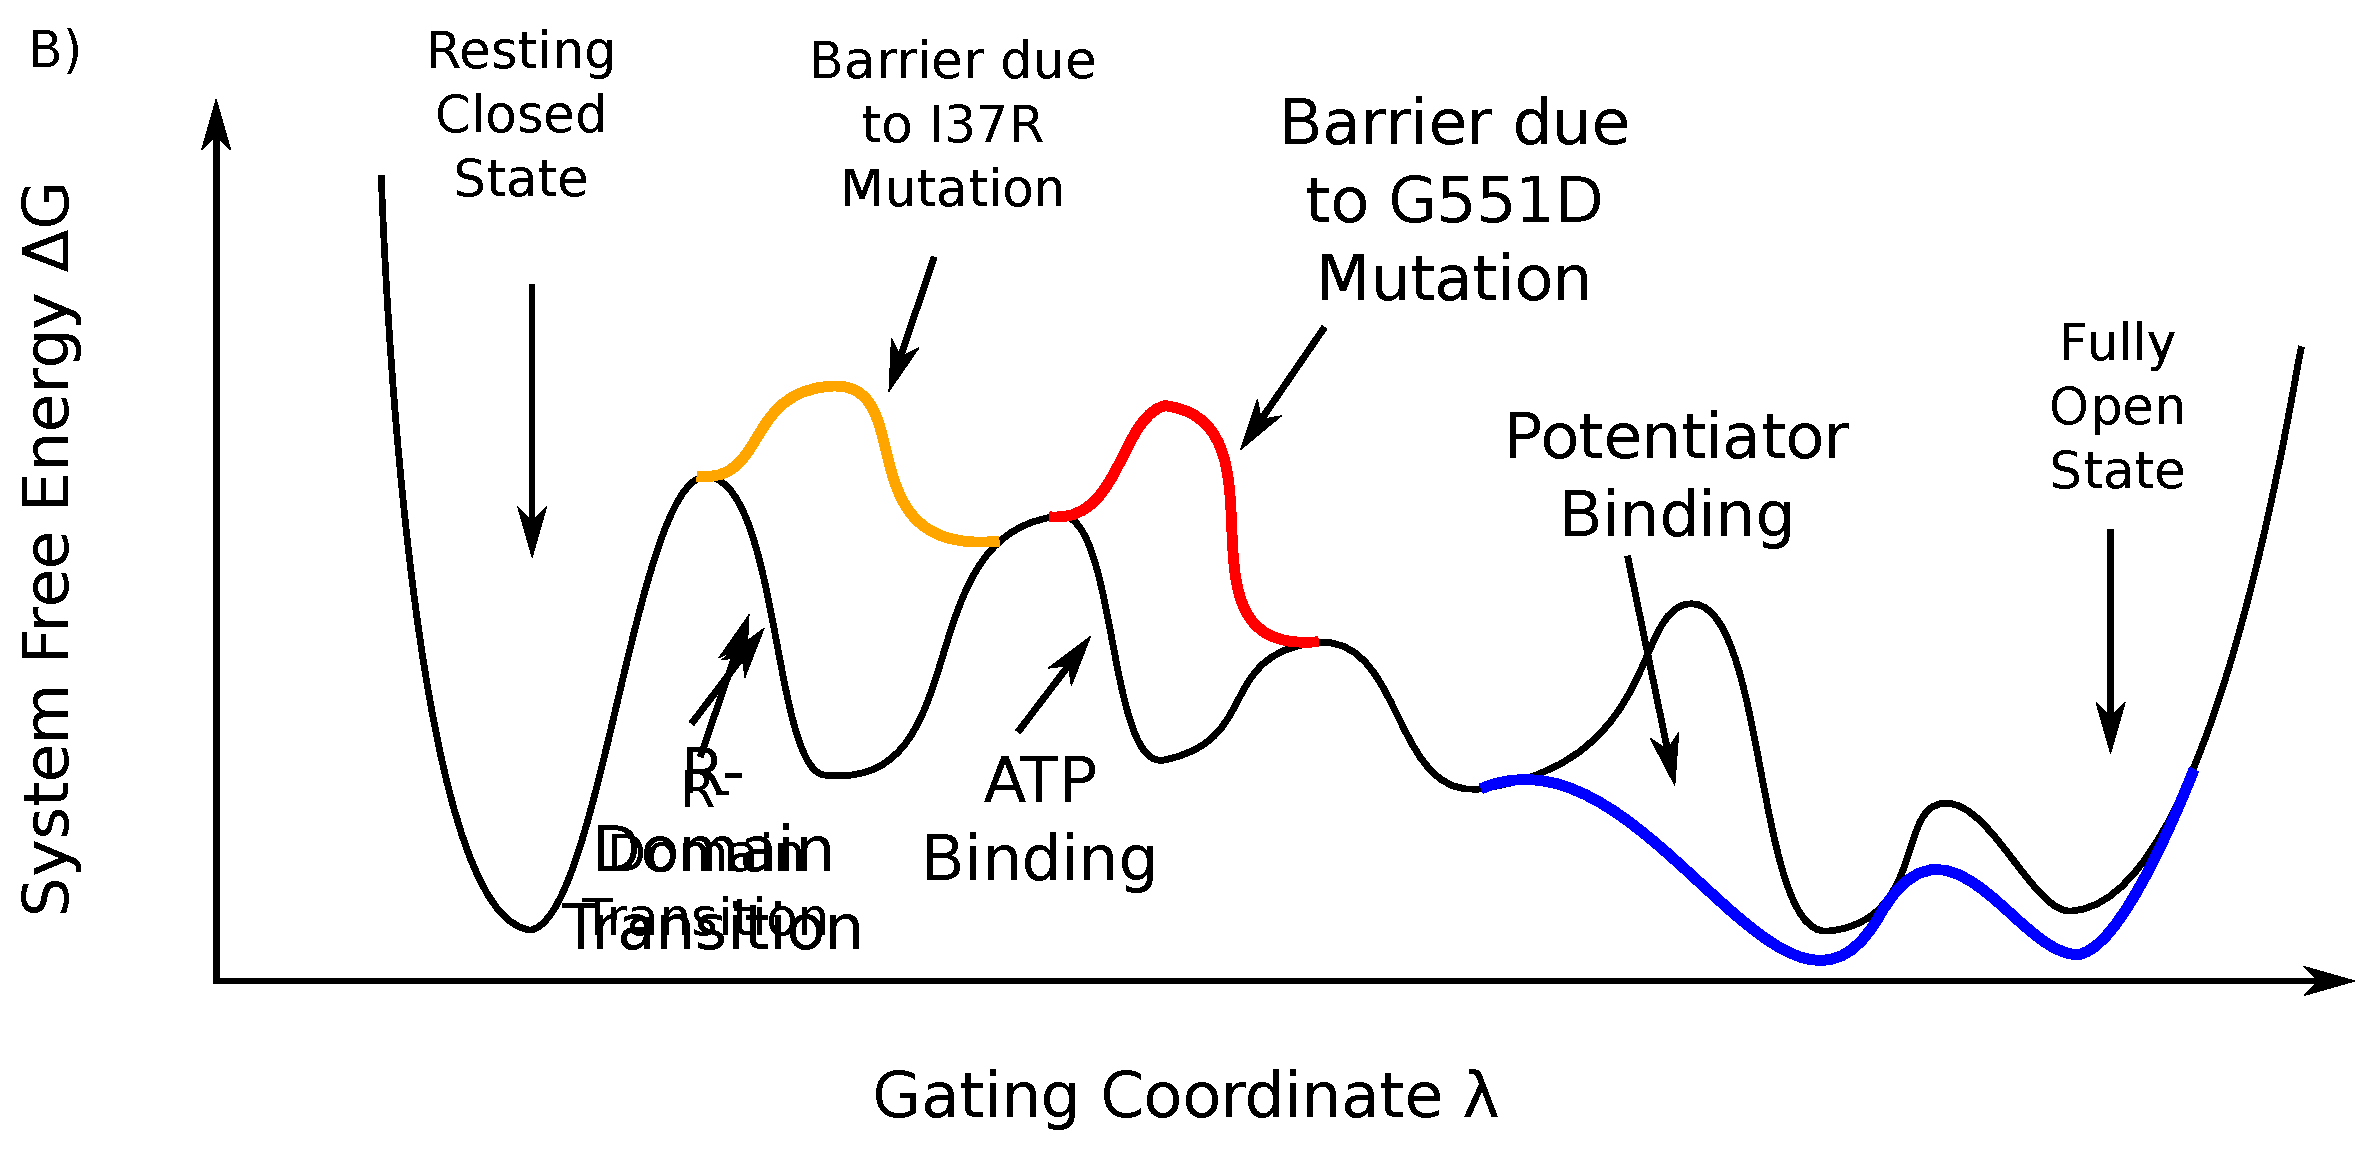
\includegraphics[width=\textwidth]{figures/drug_landscape_3.pdf}\\
	\end{center}
	\captionsetup{singlelinecheck = false, justification=raggedright}
	\caption[A physics motivated conceptual framework for how to think about the treatment of rare mutations by CFTR modulators ]{\textbf{physics motivated conceptual framework for how to think about the treatment of rare mutations by CFTR modulators}{This model was produced to explain the apparent ability of CFTR modulators to treat rare mutations with a diverse set of phenotypes. }}

\end{figure}

The ongoing discovery of rare mutations highlights the importance of this personalised approach to the treatment of CF. The process for developing potentiator class drugs was by studying the G551D mutation. Drugs that were found to restore function for this rare mutation are now widely used by sufferers of cystic fibrosis \cite{}. The study of rare mutations N1303K which currently do not respond to drugs may lead to the discovery of more effective compounds to treat cystic fibrosis such as. Thus, the approach to the treatment of Cystic Fibrosis is intersectional, as more rare mutations are discovered and treated the better the outcomes for all patients with Cystic Fibrosis will be. Each rare mutation sheds light on the function of CFTR and lets us understand and treat the root cause of the disease better.


This model makes clear what the pressing questions are in molecular cystic fibrosis research. These are three, primarily. Firstly and fundamentally, there is the task of finding the molecular details of the functional landscape in figure \ref{drug_action_figure}. Secondly, there is the elucidation of molecular misfunction of mutations. We must find \textit {where} in the functional landscape these mutations are causing issues, which will also tell us how. This will allow us to meaningfully group mutations into molecular theratypes. This leads us to the final task: Finding drugs to treat each of these theratypes. My personal opinion for the direction of each of these tasks is layed out in the subsequent sections.

Should the above model prove successful, such an approach approach to personalised medicine could  be considered when studying other monogenic diseases such as Muscular  Dystrophy, Sickle Cell Anemia and Huntington's disease \cite{}. Once single genes are understood the understanding could be built outward to encompass more complex diseases which involve the interactions between many genes such as diabetes and cancer. The future of personalised medicine is bright and it is possible that much of its breakthroughs will come from the molecular level.

\section{Outstanding fundamental questions about CFTR Function}
Firstly, there are controversies surrounding the structure of this protein. Primarily determining resolving the physiologically relevant conformations of TM8 and the conduction pathway of ions through CFTR.

Secondly, there are questions about how tightly the coupling of hydrolysis of ATP in the NBDs is to the conduction of ions.

\section{Grouping of Theratypes}
\begin{figure}
	\begin{center}
	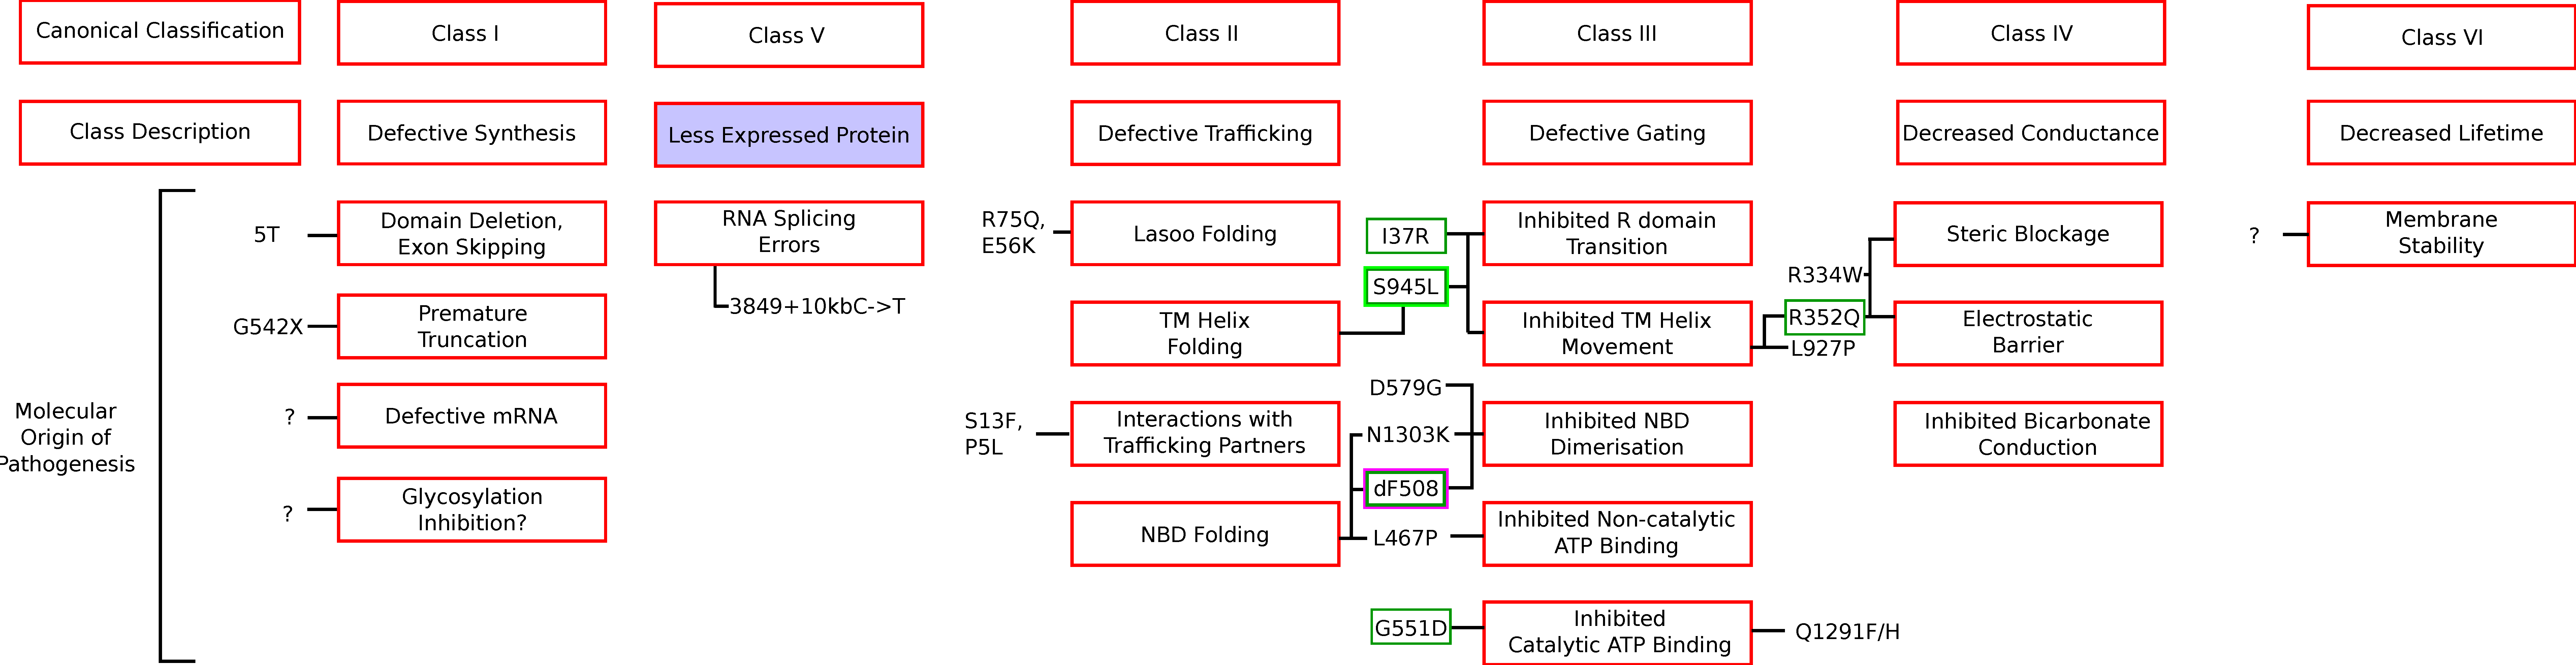
\includegraphics[angle=90,origin=c,width=0.35\textwidth]{figures/classes_mutations.pdf}\\
	%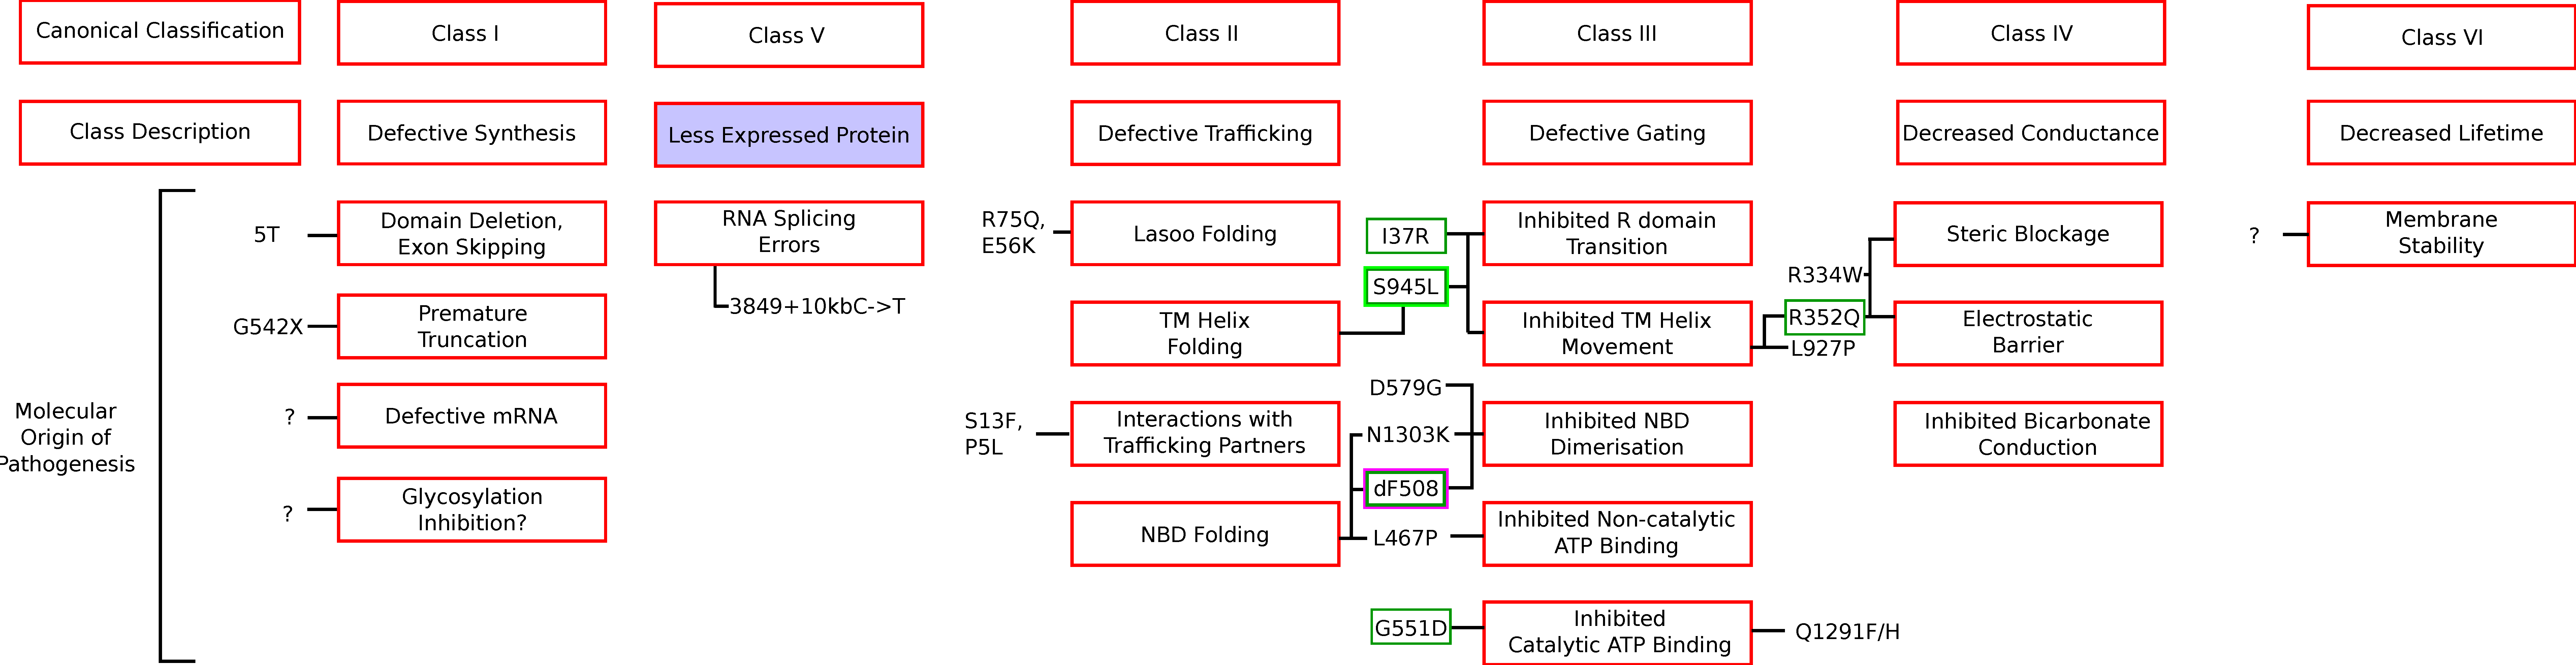
\includegraphics[width=\textwidth]{figures/classes_mutations.pdf}\\
	\end{center}
	\captionsetup{singlelinecheck = false, justification=raggedright}
	\caption[Granular grouping of CF pathogenesis]{\textbf{Granular Grouping of Cystic Fibrosis Causing Mutations}{ Conventionally, CF genotypes are grouped into 7 classes of phenotype. These 7 classes, while useful are broad when one notes that the molecular details of misfunction can in fact be due to an array of factors. By realising that classification into a given class can be due to different factors we can gain a more complete  picture of the molecular cause of CF by delineating the molecular fingerprint of each mutation.}}

\end{figure}

As outlined in figure \ref{mutation_classes_figure} earlier, the molecular fingerprint of a mutation can be quite complex and ongoing work is needed to meaningfully group these mutations into more clinically meaningful categories. My prediction is that the conventional 6 classes will be more and more finely defined in order to choose CFTR modulators which are more specific to a patient's genotype and epithelial phenotype. 

\section{Resolving Drug Action}
Closely related to the above two categories is the mechanism of action for existing drugs and the development of new drugs. The reason we were able to discover potentiator class drugs is through the study of a rare mutation. High throughput screening of small molecules in restoring the gating class mutation G551D led to the discovery of gating class drugs. In this way we can see how the study of rare CF can lead to better outcomes for all sufferers of the disease. This is especially pertinent as more rare genotypes are discovered in non-Caucasian populations such as in Asia and the Middle East. 

Additionally, it should be obvious from this work that the action of these drugs is are highly dependent on the molecular function of CFTR. These small molecule drugs \textit{select} for a physiologically present conformation, so we would wish to design molecules which select for conformations which deliver the most clinic benefit. This is non-trivial and I believe  combination of careful molecular experiments, such as those of from the laboratories of Tzyh-Chang Hwang,  Christine E. Bear, L\'aszl\'o Csan\'ady and Paul Linsdell \cite{linsdell2018, csanady2019, zhang2017b}, and molecular simulations such as those found in this thesis and studies from the labs of John Paul Monron and Isabelle Callebaut \cite{Hoffmann2018}.
